\documentclass[11pt,letterpaper]{article}
\usepackage{array}
\usepackage{fullpage}
\usepackage{graphicx}
\usepackage{parskip}
\usepackage{amsmath}
\usepackage[small]{caption}
\usepackage{graphpap}
\usepackage{logpap}
\usepackage{tabularx}
\usepackage{url}
\usepackage{hyperref}
\usepackage{enumitem}

\renewcommand{\thesection}{PART \arabic{section}: }

\newcounter{question}[section]
\newenvironment{question}[1][]{\refstepcounter{question}\par\medskip
   \textbf{\arabic{section}.\thequestion.} \rmfamily}{\medskip}

\usepackage{titlesec}
\titleformat{\section}{\clearpage\normalfont\bfseries}{\thesection}{0em}{}
\titlespacing{\section}{0pt}{0.5\baselineskip}{0pt}

\titleformat{\subsection}[runin]
{\normalfont\bfseries}{\thesubsection}{1em}{}

\titleformat{\subsubsection}{\normalfont\bfseries}{\thesubsubsection}{0em}{}
\titlespacing{\subsubsection}{0pt}{0.5\baselineskip}{0pt}

\newcounter{saveenumi}
\newcommand{\seti}{\setcounter{saveenumi}{\value{enumi}}}
\newcommand{\conti}{\setcounter{enumi}{\value{saveenumi}}}

\usepackage[dvipsnames]{xcolor}
\newcommand{\sol}[1]{{\color{NavyBlue} #1}}



\begin{document}
\setlength{\parindent}{0in}
\setlength{\itemsep}{0in}
%% EQUIP: Force Probe, Pulley, Track, hanger, Weight, Tilt, Scale

\begin{flushright}
PHYS S211\\
Lab 3: Forces\\
9/20/22 (due 9/27/22)
\end{flushright}

Name(s):\\

\subsubsection*{Topics:}
\begin{enumerate}
\setlength{\parskip}{3pt}
\item Familiarity with the force probe
\item Using gravity to cause horizontal cart motion
\item Frictional forces
\item Balancing masses with an inclined plane
\end{enumerate}

\subsubsection*{Introduction:}
This lab explores the relationship between forces and motion. It uses many of the same techniques and equipment from previous lectures and labs. In the lab you will (i) measure the force applied to a small cart while graphically displaying that force along with the cart's resulting motion, (ii) estimate the coefficient of friction of a sliding block, and (iii) determine the mass needed to hold a cart on a ramp in static equilibrium.

Forces are vector quantities that influence the motion of an object. In the first part of the lab you will simply explore the relationship between forces and motion. In the second and third parts of the lab you will deal with the following forces:
\begin{itemize}
\setlength{\parskip}{3pt}
\item Gravitational force, $F_g = mg$ for object's near the Earth's surface; points straight downward
\item Normal force, $F_n$, points perpendicular to surfaces and prevents objects from passing through each other
\item Tensional force, $F_t$, points parallel to a string or rope and pulls on objects
\item Force of kinetic friction, $F_k=\mu_kF_n$ where $\mu_k$ is the coefficient of kinetic friction, points opposite the direction of motion
\end{itemize}


\subsubsection*{What you should turn in:}
\begin{itemize}
\setlength{\parskip}{3pt}
\item Part 1: Plots of position, velocity, acceleration, and force from one experiment [2 pts].
\item Part 1: Plot of mean force vs. mean acceleration (derived from several experiments) [2 pts].
\item Part 1: Discussion of the plots [4 pts].
\item Part 2: Deriviation relating the coefficient of friction of the sliding block to the mass of the block, the mass of falling weight, and the acceleration of the system. Plug in your measured values to estimate the coefficient of friction. [4 pts]
\item Part 3: Free-body diagram [2 pts], derivations and calculations [4 pts], and a description of the experiment [2 pts].
%\item Part 3: Free-body diagram (2 pts), derivations and calculations (4 pts), and a photo of the experiment (2 pts).
\end{itemize}
You may submit a group report. The next lab will require a formal report (details to come). 

\subsubsection*{Equipment:}
\begin{itemize}
\setlength{\parskip}{3pt}
\item LabQuest interface, cables, and motion sensor
\item Track, motion cart, force probe, pulley, string, friction block, mass hanger and various masses
\item Inclined plane
\end{itemize}



\section{HORIZONTAL ACCELERATION} 
Plug the Force Probe and the Motion Probe into the LabQuest logger. Make sure the sensors are properly calibrated. In other words, make sure that you trust the numbers that the probes and computer are telling you. Does the force probe read zero when there is zero force?

Next, using a string and table mounted pulley, set-up the cart, force probe, and bench as illustrated:

\begin{figure}[h]
\begin{center}
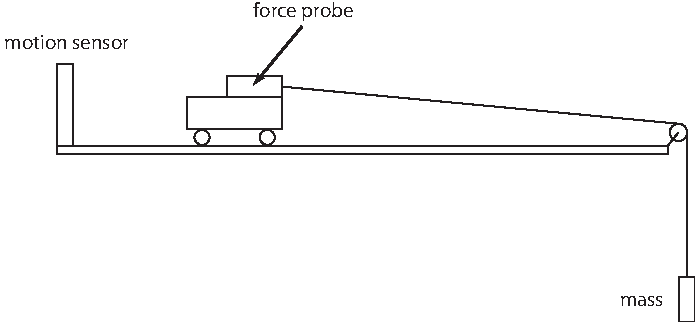
\includegraphics[]{./cart_and_pulley}
\end{center}
\end{figure}


Hanging 300~g produces a gravitational force of 2.94 N.  Check that this is what the force probe reads, keeping in mind that the hanger has a mass of 50~g.  What is the precision of the scale? How accurate is the force probe?  Using the Live Readout values at the bottom of the graph, check the calibration. Add mass to the hanger and check the measured force.  Does changing the orientation of the probe (to vertical, for example) change the measured value of force? Why? You do not need to answer these questions in your lab report, but do keep them in mind when analyzing and plotting the data that you collect.

Now using the cart, pulley, and weights, you will use the motion probe and force probe to explore the relationship between force and acceleration. Collect both motion and force data for the cart as it accelerates away from the motion sensor (use measurements at distances greater than about 50 cm from the motion sensor for the best results).  Using the position-time graph, select the data before you released the cart and ``Strike Through Data Cells'' under the Edit menu.  Similarly mark out the data after the cart reached the end of the track.  Adjust the time axis to zoom in on this subset of the data.  Can you reliably measure the acceleration with the motion sensor?  Try using the slope of the velocity curve to make a better estimate of the
acceleration. Use either the button marked ``M=?'' to find the instantaneous slope of the line or the button marked ``R=?'' to find the mean slope over a time interval. \textbf{Include in your report plots of position, velocity, acceleration, and force vs. time from one experiment, produced using MATLAB.}% Also include a plot of force vs. acceleration.}  

Next, using different masses on the hanger, measure five different sets of force (mean force) and acceleration (mean acceleration) pairs. Make a plot of your measured force ($y$-axis) vs. acceleration ($x$-axis). 

Here's how to do it in MATLAB:
\begin{verbatim}>> force=[F1 F2 F3 F4 F5]; % enter your force measurements F1, F2, etc. \end{verbatim}
\begin{verbatim}>> acceleration=[a1 a2 a3 a4 a5]; % enter your acceleration measurements; \end{verbatim}
\begin{verbatim}>> p=polyfit(acceleration,force,1); \end{verbatim}
\begin{verbatim}>> plot(acceleration,force,acceleration,p(1)*acceleration+p(2)) \end{verbatim}

The \verb+polyfit+ command used above fits a first-order polynomial (a line) to the data and returns two coefficients. \verb+p(1)+ gives the slope of the line. Note that you always get information about a MATLAB command by typing, e.g., 
\begin{verbatim}>> help polyfit\end{verbatim}

 \textbf{Submit this plot}.  What are the units of the slope?  What does the value of the slope of this plot correspond to physically? What is the y-intercept, and what is its signficance?

Check with me that you understand the relationship between the force acting on the cart and the motion of the cart before continuing on to Parts 2 and 3.

\section{FRICTION}
In this part of the lab you will measure the coefficient of friction between a block and the track. Use the same set-up as in Part 1, except replace the cart with one of the friction blocks. Do not use the force probe or motion sensor. Measure the mass of the block and the distance that the block slides, which will be the same as the distance that the hanging mass falls. Record the amount of time that it takes the hanging mass to fall to the floor, and then use kinematics to determine it's acceleration. Using this acceleration and what you learned about forces in Part 1, write down a system of equations involving forces and solve for the coefficient of kinetic friction. You should assume that tensional force acting on the block and the tensional force acting on the falling mass have the same magnitude.

\textbf{Submit a derivation showing how you estimated the coefficient of friction. Indicate what you measured for the acceleration and mass of the block, and calculate the coefficient of friction.} 

\section{INCLINED PLANE}
For the third part of the lab, use the inclined plane apparatus.  The inclined plane has a device for measuring angles and a pulley at one end. Add some mass to the cart and measure, using a scale, the total mass of the cart. Select an angle to tilt the plane.  Draw the free body diagram of the apparatus and \textbf{include the diagram in your report}.

Using what you learned in Parts 1 and 2, calculate the mass needed to counter-balance the mass of the cart. In doing so you need to keep in mind that forces are vectors, and therefore you need to be careful when adding or subtracting forces. \textbf{Show the equations that you used}. Put this mass on the hanger and test your calculation. What happens if you put an ever so slightly heavier or lighter mass on the hanger? Does the cart move? Why or why not? Discuss the results.

If you increase the mass of the cart by 200~g, what is the new mass that you need on the hanger?  Test this set-up and discuss. You may have to find creative ways to add mass to the cart; one way is to put additional mass on the string just above the cart.

If you double (or halve, whatever is appropriate for your initial
angle) the angle, what is the new value of the mass that you need to balance the cart?  Test this set-up and discuss.
 
\textbf{Write one to two paragraphs describing the experiment and your results.}

%\clearpage
%\textbf{\MakeUppercase{Part 3: Tensional forces and vectors}}\\
%In the last part of the lab you will use a force table and pulleys to explore the tensional force. Set-up the force table and level it as best as you can. Attach three pulleys to the force table at angles of 10$^\circ$, 135$^\circ$. Next, attach three strings and hangars to the small ring. If you place an additional 50 g and 100 g on the first two pulleys (i.e., those at 10$^\circ$ and 135$^\circ$, respectively), where should you place the third pulley and how much mass should you hang over it in order to get the system into static equilibrium?

%Solve this using theoretical arguments, and then test your answer using the force plate. Submit (i) a free body diagram, (ii) your derivation, and (iii) a photo of your system in static equilibrium.
\end{document}
